\paragraph{La classe ProxyGUI}

\begin{minipage}
    {\linewidth}
    \centering
    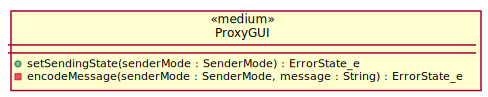
\includegraphics[width=0.65\linewidth]{../schemas/Conception_detaillee/classe_proxyGUI.pdf}
    \captionof{figure}{Diagramme de classe de ProxyGUI}
\end{minipage}

\subparagraph{Philosophie de conception \newline} 

\medspace

La classe ProxyGUI qui est dans le programme {\nomLogiciel} a pour rôle de simuler le comportement de la classe GUI présente dans l'application {\nomApplication}. Toutes les requêtes que Sender doit envoyer à GUI passent par cette classe.

\subparagraph{Description structurelle \newline}

\medspace

\textbf{Attributs :}

N.A.

\textbf{Services offerts :}

\begin{itemize}
    \item \textbf{setSendingState(senderMode : SenderMode) : ErrorState\_e} --- Opération qui permet de définir l'état du Mode Envoi du système.
    \item \textbf{encodeMessage(senderMode : SenderMode, message : String) : ErrorState\_e} --- Opération qui permet d'encoder un état du Mode Envoi en une chaine de caractère.
\end{itemize}
